%package list
\documentclass{article}
\usepackage[top=3cm, bottom=3cm, outer=3cm, inner=3cm]{geometry}
\usepackage{multicol}
\usepackage{graphicx}
\usepackage{url}
%\usepackage{cite}
\usepackage{hyperref}
\usepackage{array}
%\usepackage{multicol}
\newcolumntype{x}[1]{>{\centering\arraybackslash\hspace{0pt}}p{#1}}
\usepackage{natbib}
\usepackage{pdfpages}
\usepackage{multirow}
\usepackage[normalem]{ulem}
\useunder{\uline}{\ul}{}
\usepackage{svg}
\usepackage{xcolor}
\usepackage{listings}
\lstdefinestyle{ascii-tree}{
    literate={├}{|}1 {─}{--}1 {└}{+}1 
  }
\lstset{basicstyle=\ttfamily,
  showstringspaces=false,
  commentstyle=\color{red},
  keywordstyle=\color{blue}
}
%\usepackage{booktabs}
\usepackage{caption}
\usepackage{subcaption}
\usepackage{float}
\usepackage{array}

\newcolumntype{M}[1]{>{\centering\arraybackslash}m{#1}}
\newcolumntype{N}{@{}m{0pt}@{}}


%%%%%%%%%%%%%%%%%%%%%%%%%%%%%%%%%%%%%%%%%%%%%%%%%%%%%%%%%%%%%%%%%%%%%%%%%%%%
%%%%%%%%%%%%%%%%%%%%%%%%%%%%%%%%%%%%%%%%%%%%%%%%%%%%%%%%%%%%%%%%%%%%%%%%%%%%
\newcommand{\itemEmail}{jccahuanala@unsa.edu.pe}
\newcommand{\itemStudent}{Joshep Antony Ccahuana Larota}
\newcommand{\itemCourse}{Programación Web 2}
\newcommand{\itemCourseCode}{20223010}
\newcommand{\itemSemester}{III}
\newcommand{\itemUniversity}{Universidad Nacional de San Agustín de Arequipa}
\newcommand{\itemFaculty}{Facultad de Ingeniería de Producción y Servicios}
\newcommand{\itemDepartment}{Departamento Académico de Ingeniería de Sistemas e Informática}
\newcommand{\itemSchool}{Escuela Profesional de Ingeniería de Sistemas}
\newcommand{\itemAcademic}{2023 - A}
\newcommand{\itemInput}{Del 30 mayo 2023}
\newcommand{\itemOutput}{Al 09 junio 2023}
\newcommand{\itemPracticeNumber}{04}
\newcommand{\itemTheme}{Python}
%%%%%%%%%%%%%%%%%%%%%%%%%%%%%%%%%%%%%%%%%%%%%%%%%%%%%%%%%%%%%%%%%%%%%%%%%%%%
%%%%%%%%%%%%%%%%%%%%%%%%%%%%%%%%%%%%%%%%%%%%%%%%%%%%%%%%%%%%%%%%%%%%%%%%%%%%

\usepackage[english,spanish]{babel}
\usepackage[utf8]{inputenc}
\AtBeginDocument{\selectlanguage{spanish}}
\renewcommand{\figurename}{Figura}
\renewcommand{\refname}{Referencias}
\renewcommand{\tablename}{Tabla} %esto no funciona cuando se usa babel
\AtBeginDocument{%
	\renewcommand\tablename{Tabla}
}

\usepackage{fancyhdr}
\pagestyle{fancy}
\fancyhf{}
\setlength{\headheight}{30pt}
\renewcommand{\headrulewidth}{1pt}
\renewcommand{\footrulewidth}{1pt}
\fancyhead[L]{\raisebox{-0.2\height}{
\includegraphics[width=3cm]{img/logo_episunsa.png}}}
\fancyhead[C]{\fontsize{7}{7}\selectfont	\itemUniversity \\ \itemFaculty \\ \itemDepartment \\ \itemSchool \\ \textbf{\itemCourse}}
\fancyhead[R]{\raisebox{-0.2\height}{
\includegraphics[width=1.2cm]{img/logo_abet}}}
\fancyfoot[L]{Estudiante Joshep Ccahuana Larota}
\fancyfoot[C]{\itemCourse}
\fancyfoot[R]{Página \thepage}

% para el codigo fuente
\usepackage{listings}
\usepackage{color, colortbl}
\definecolor{dkgreen}{rgb}{0,0.6,0}
\definecolor{gray}{rgb}{0.5,0.5,0.5}
\definecolor{mauve}{rgb}{0.58,0,0.82}
\definecolor{codebackground}{rgb}{0.95, 0.95, 0.92}
\definecolor{tablebackground}{rgb}{0.8, 0, 0}

\lstset{frame=tb,
	language=bash,
	aboveskip=3mm,
	belowskip=3mm,
	showstringspaces=false,
	columns=flexible,
	basicstyle={\small\ttfamily},
	numbers=none,
	numberstyle=\tiny\color{gray},
	keywordstyle=\color{blue},
	commentstyle=\color{dkgreen},
	stringstyle=\color{mauve},
	breaklines=true,
	breakatwhitespace=true,
	tabsize=3,
	backgroundcolor= \color{codebackground},
}

\begin{document}
	
	\vspace*{10px}
	
	\begin{center}	
		\fontsize{17}{17} \textbf{ Informe de Laboratorio \itemPracticeNumber}
	\end{center}
	\centerline{\textbf{\Large Tema: \itemTheme}}
	%\vspace*{0.5cm}	

	\begin{flushright}
		\begin{tabular}{|M{2.5cm}|N|}
			\hline 
			\rowcolor{tablebackground}
			\color{white} \textbf{Nota}  \\
			\hline 
			     \\[30pt]
			\hline 			
		\end{tabular}
	\end{flushright}	

	\begin{table}[H]
		\begin{tabular}{|x{4.7cm}|x{4.8cm}|x{4.8cm}|}
			\hline 
			\rowcolor{tablebackground}
			\color{white} \textbf{Estudiante} & \color{white}\textbf{Escuela}  & \color{white}\textbf{Asignatura}   \\
			\hline 
			{\itemStudent \par \itemEmail} & \itemSchool & {\itemCourse \par Semestre: \itemSemester \par Código: \itemCourseCode}     \\
			\hline 			
		\end{tabular}
	\end{table}		
	
	\begin{table}[H]
		\begin{tabular}{|x{4.7cm}|x{4.8cm}|x{4.8cm}|}
			\hline 
			\rowcolor{tablebackground}
			\color{white}\textbf{Laboratorio} & \color{white}\textbf{Tema}  & \color{white}\textbf{Duración}   \\
			\hline 
			\itemPracticeNumber & \itemTheme & 04 horas   \\
			\hline 
		\end{tabular}
	\end{table}
	
	\begin{table}[H]
		\begin{tabular}{|x{4.7cm}|x{4.8cm}|x{4.8cm}|}
			\hline 
			\rowcolor{tablebackground}
			\color{white}\textbf{Semestre académico} & \color{white}\textbf{Fecha de inicio}  & \color{white}\textbf{Fecha de entrega}   \\
			\hline 
			\itemAcademic & \itemInput &  \itemOutput  \\
			\hline 
		\end{tabular}
	\end{table}
	
	\section{Tarea}
	\begin{itemize}		
		\item Implemente los métodos de la clase Picture. Se recomienda que implemente la clase picture por etapas, probando realizar los dibujos que se muestran en la siguiente preguntas.
		\item Usando únicamente los métodos de los objetos de la clase Picture, dibuje las figuras (invocando el método "draw()").
	\end{itemize}
		
	\section{Equipos, materiales y temas utilizados}
	\begin{itemize}
		\item Sistema operativo Windows 11.
		\item Librería PyGame.
		\item Python 3.10.11.
		\item Git 2.39.2.
		\item Cuenta en GitHub con el correo institucional (Joshep-c).
		\item TextMaker / MikTex
		\item Programación Orientada a Objetos.
		\item Manejo de matrices unidimensionales.
	\end{itemize}
	
	\section{URL de Repositorio Github}
	\begin{itemize}
		\item URL del Repositorio GitHub para clonar o recuperar.
		\item \url{https://github.com/Joshep-c/PW2LAB.git}
		\item URL para el laboratorio 04 en el Repositorio GitHub.
		\item \url{https://github.com/Joshep-c/PW2LAB/tree/68f2e2f2197a1bb6bfe93bfcbef903c246a52603/Python}
	\end{itemize}
	
	\section{Implementación de los métodos}
	
	\subsection{Método \textit{verticalMirror()}}
	Se modifica la variable de retorno del método, por un Picture, y ya no un List.
		
	\lstinputlisting[language=Python, caption={verticalMirror.py},numbers=left,]{src/verticalMirror.py}
		
	\subsection{Método \textit{horizontalMirror()}}
		
	El siguiente método toma como parámetro un Picture, en la cual recorre de manera inversa la lista “[::-1]”, para después almacenarla en otra. Y retornar otro Picture.
		
	\lstinputlisting[language=Python, caption={horizontalMirror.py},numbers=left,]{src/horizontalMirror.py}
		
	\subsection{Método \textit{negative()}}
	
	En este método el Picture recibido por el parámetro, se recorre cada elemento, y con un sub for cada caracter es cambiado de color mediante el metodo "\_invColor()", despues cada el valor del color nuevo es almacenado en conjunto en una nueva lista, que posteriormente es transformada en Picture y se retorna.
	
	\lstinputlisting[language=Python, caption={negative.py},numbers=left,]{src/negative.py}
	
	\subsection{Método \textit{join()}}
	
	La función de este método era poder fusionar dos imágenes en una, colocando en la derecha la imagen recibida (p). Para lograr esto,  se convirtió las imágenes en arrays con el .img para luego agregar ambos en un array new\_img.
	
	\lstinputlisting[language=Python, caption={join.py},numbers=left,]{src/join.py}
	
	\subsection{Método \textit{up()}}
	
	El funcionamiento del método se basa en la agregación de un nuevo Picture por encima del inicial, como los Picture.img, son listas se puede lograr con una simple agregación con “+”.
	
	\lstinputlisting[language=Python, caption={up.py},numbers=left,]{src/up.py}
	
	\subsection{Método \textit{under()}}
	
	De igual manera que el anterior método, pero invirtiendo los dos picture, para que el picture “p” quede por debajo del instanciado.
	
	\lstinputlisting[language=Python, caption={under.py},numbers=left,]{src/under.py}
	
	\subsection{Método \textit{horizontalRepeat()}}
	
	Haciendo uso de un bucle for, modificado para recorrer mediante una numeración ya que el parámetro ingresado es un entero, se va repitiendo la misma funcionalidad del método join(), agregando como argumento el mismo Picture instanciado al momento de su llamado.
	
	\lstinputlisting[language=Python, caption={horizontalRepeat.py},numbers=left,]{src/horizontalRepeat.py}
	
	\subsection{Método \textit{verticalRepeat()}}
	
	El método tiene la misma base de funcionamiento que el anterior, pero como se busca la repetición de un Picture de manera vertical, se hace uso del método “up()” implementado anteriormente.
	
	\lstinputlisting[language=Python, caption={verticalRepeat.py},numbers=left,]{src/verticalRepeat.py}
	
	\subsection{Método \textit{rotate()}}
	
	Este método cambia las posiciones de la lista .img del Picture, ósea obteniendo cada carácter en el eje “y”, se coloca de manera que esté en el eje “x” en una nueva lista, que posteriormente se retorna como Picture.
	
	\lstinputlisting[language=Python, caption={rotate.py},numbers=left,]{src/rotate.py}
	
	\clearpage
	
	\section{Ejecuciones y código}
	
	\subsection{Ejercicio A:}
	
	En el siguiente código se crea las dos primeras líneas por separado, la primera generando un Picture con un caballo negro que se coloco al costado e un caballo blanco, de manera contaaria la segunda fila, y finalmente se coloca uno debajo del otro con el método under.
	
	\begin{figure}[H]
		\centering
		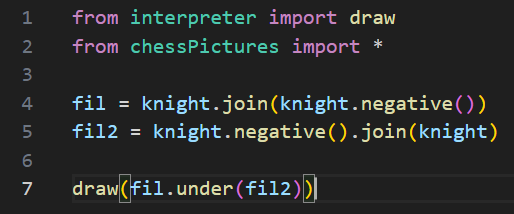
\includegraphics[width=0.55\textwidth,keepaspectratio]{img/cap10.png}
		%\includesvg{img/automata.svg}
		%\label{img:mot2}
		%\caption{Product backlog.}
	\end{figure}	
	
	\begin{figure}[H]
		\centering
		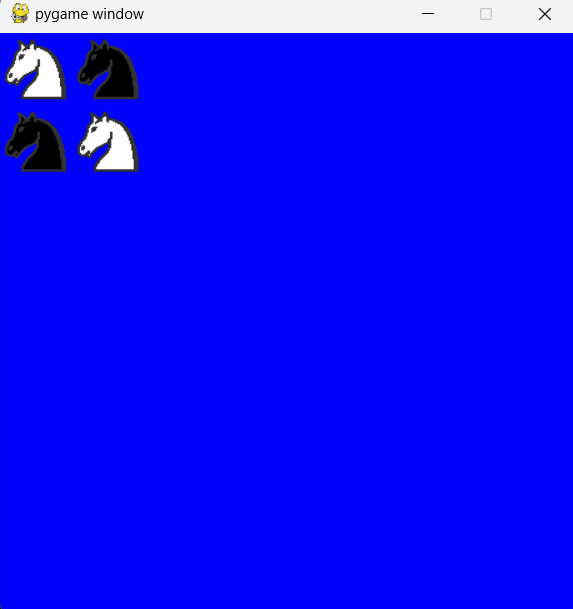
\includegraphics[width=0.55\textwidth,keepaspectratio]{img/Picture A.png}
		%\includesvg{img/automata.svg}
		%\label{img:mot2}
		%\caption{Product backlog.}
	\end{figure}	
	
	\subsection{Ejercicio B:}
	
	En este ejercicio, se inicia con la primera linea de caballos, se inserta en un caballo negro al lado derecho de un caballo negro, despues se obtiene un Picture con el método verticalMirror. Después el primer picture es colocado por encima del segundo Picture, con el método under.
	
	\begin{figure}[H]
		\centering
		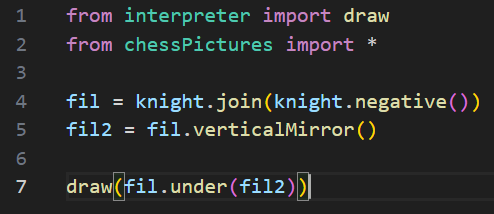
\includegraphics[width=0.55\textwidth,keepaspectratio]{img/cap11.png}
		%\includesvg{img/automata.svg}
		%\label{img:mot2}
		%\caption{Product backlog.}
	\end{figure}
	
	\begin{figure}[H]
		\centering
		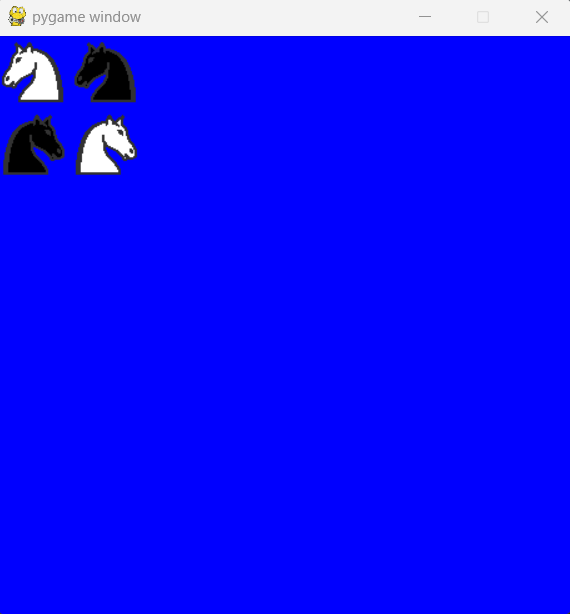
\includegraphics[width=0.55\textwidth,keepaspectratio]{img/Picture B.png}
		%\includesvg{img/automata.svg}
		%\label{img:mot2}
		%\caption{Product backlog.}
	\end{figure}	
	
	\subsection{Ejercicio C:}
	
	Para este ejercicio se usa una pieza queen se repite mediante el método horizontalRepeat con un argumento 4, para que se repita cuatro veces y que se dibuje en la ventana.
	
	\begin{figure}[H]
		\centering
		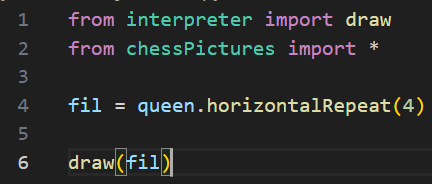
\includegraphics[width=0.55\textwidth,keepaspectratio]{img/cap12.png}
		%\includesvg{img/automata.svg}
		%\label{img:mot2}
		%\caption{Product backlog.}
	\end{figure}
	
	\begin{figure}[H]
		\centering
		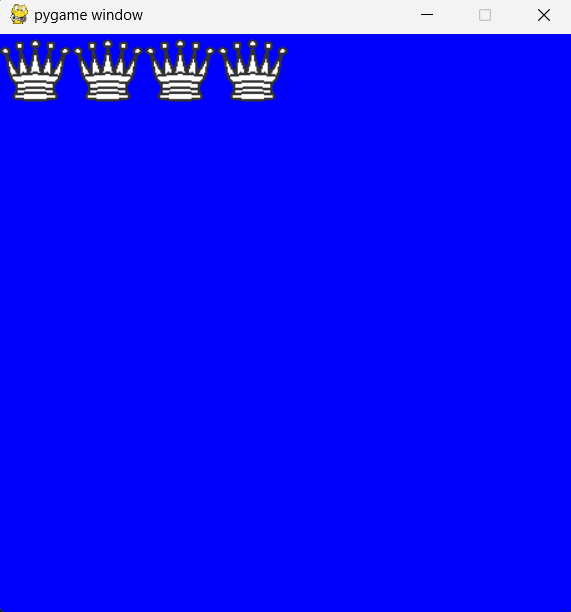
\includegraphics[width=0.55\textwidth,keepaspectratio]{img/Picture C.png}
		%\includesvg{img/automata.svg}
		%\label{img:mot2}
		%\caption{Product backlog.}
	\end{figure}	
	
	\subsection{Ejercicio D:}
	
	En el ejercicio D, primero se coloca un Picture square.negative al lado derecho de un square, para después repetir este Picture 4 veces con el método horizontalRepeat.
	
	\begin{figure}[H]
		\centering
		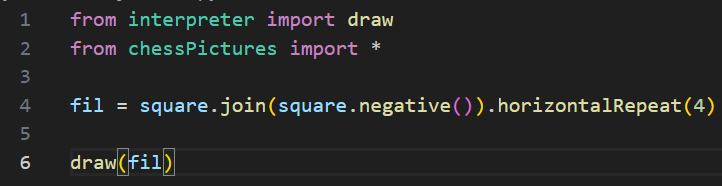
\includegraphics[width=0.55\textwidth,keepaspectratio]{img/cap13.png}
		%\includesvg{img/automata.svg}
		%\label{img:mot2}
		%\caption{Product backlog.}
	\end{figure}
	
	\begin{figure}[H]
		\centering
		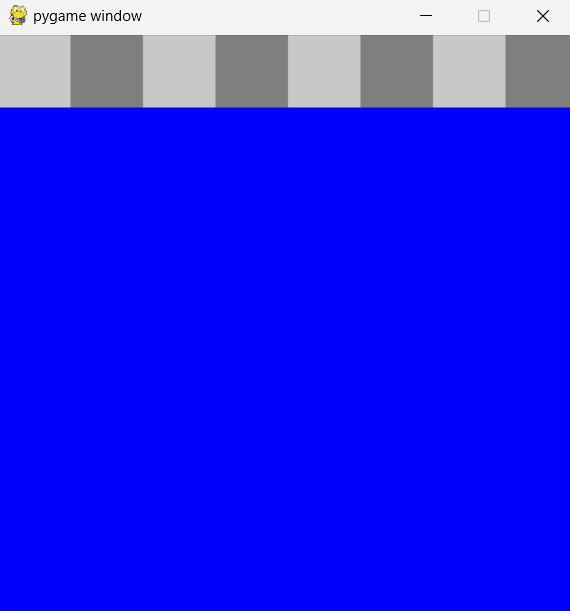
\includegraphics[width=0.55\textwidth,keepaspectratio]{img/Picture D.png}
		%\includesvg{img/automata.svg}
		%\label{img:mot2}
		%\caption{Product backlog.}
	\end{figure}	
	
	\subsection{Ejercicio E:}
	
	De igual manera con el anterior ejercicio, pero invirtiendo las posiciones de las dos primeras square.
	
	\begin{figure}[H]
		\centering
		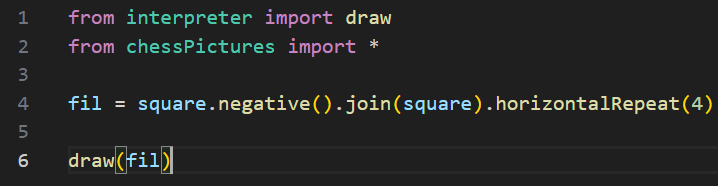
\includegraphics[width=0.55\textwidth,keepaspectratio]{img/cap14.png}
		%\includesvg{img/automata.svg}
		%\label{img:mot2}
		%\caption{Product backlog.}
	\end{figure}
	
	\begin{figure}[H]
		\centering
		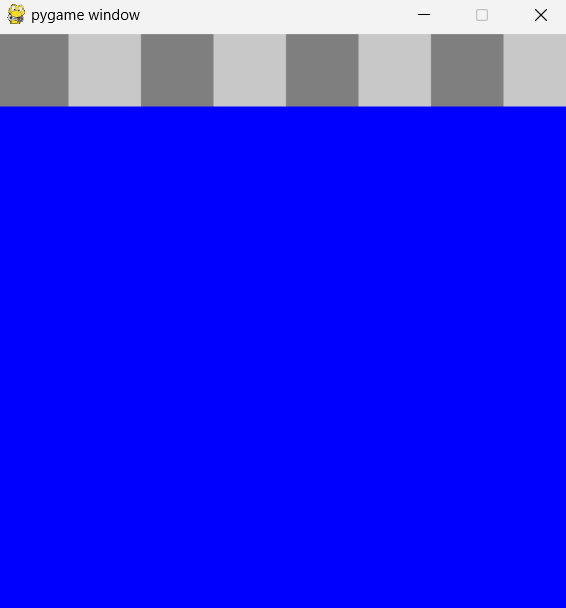
\includegraphics[width=0.55\textwidth,keepaspectratio]{img/Picture E.png}
		%\includesvg{img/automata.svg}
		%\label{img:mot2}
		%\caption{Product backlog.}
	\end{figure}	
	
	\subsection{Ejercicio F:}
	
	Utilizando los dos ejercicios anteriores, pero colocando uno debajo de otro con el método under, y duplicando de manera vertical este último Picture generado, con el método under con el argumento de si mismo.
	
	\begin{figure}[H]
		\centering
		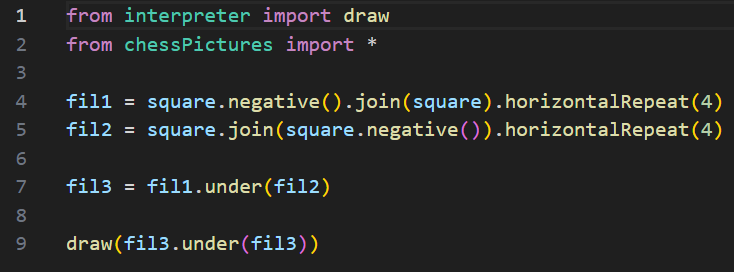
\includegraphics[width=0.55\textwidth,keepaspectratio]{img/cap15.png}
		%\includesvg{img/automata.svg}
		%\label{img:mot2}
		%\caption{Product backlog.}
	\end{figure}
	
	\begin{figure}[H]
		\centering
		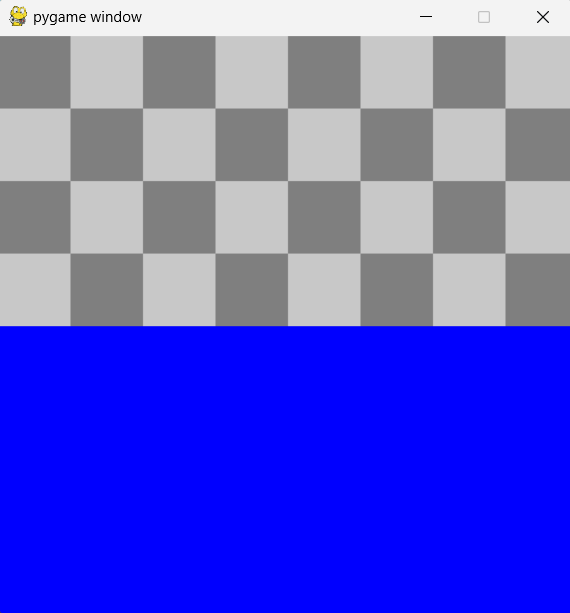
\includegraphics[width=0.55\textwidth,keepaspectratio]{img/Picture F.png}
		%\includesvg{img/automata.svg}
		%\label{img:mot2}
		%\caption{Product backlog.}
	\end{figure}	
	
	\subsection{Ejercicio G:}
	
	Aquí podemos ver las tres funciones que ayudan a la principal en la generación de las piezas y el espacio entre las piezas negras y blancas.
	
	add\_pawn: genera una imagen con los 8 peones (pawn) de manera horizontal y de color blanco (por defecto).
	
	negative\_pieces: recibe un list por argumento y recorre cada uno de los Picture para volver para modificar cada uno y volverlo negativo, para después almacenarlo en una nueva lista y retorna esta (arr\_negative).
	
	add\_main\_list: esta función tiene como propósito generar una lista con los Pieces principales (con excepción de los peones), para después retornar	esta lista (main\_list).
	
	\begin{figure}[H]
		\centering
		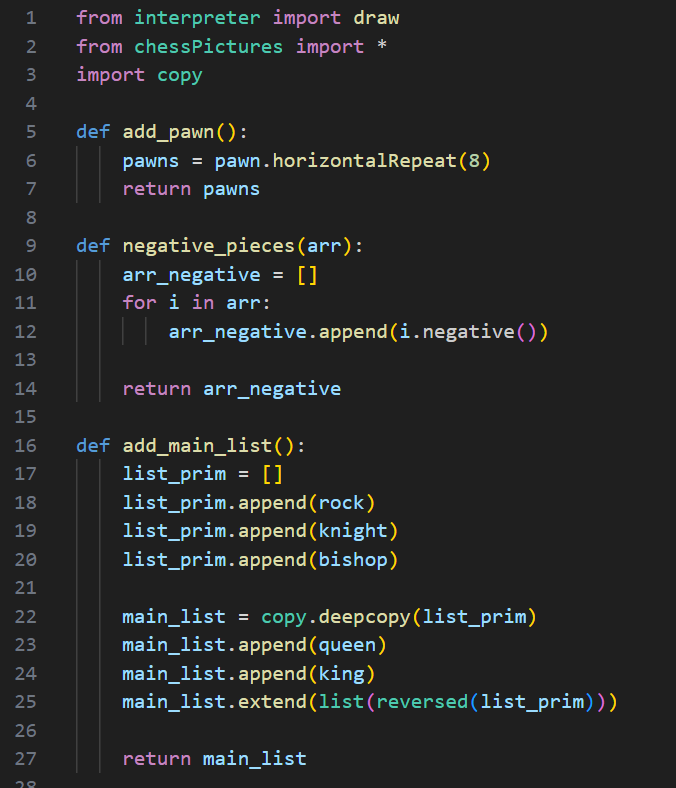
\includegraphics[width=0.55\textwidth,keepaspectratio]{img/cap16_1.png}
		%\includesvg{img/automata.svg}
		%\label{img:mot2}
		%\caption{Product backlog.}
	\end{figure}
	
	Esta es la función principal “add\_pieces” donde se crean un Picture con los peones, una lista con las piezas principales en blanco (método add\_main\_list), después se crea un Picture y lista nuevos negros usando lo anteriormente creado. Para después mediante un for ingresar cada elemento de la lista de piezas negras a un Picture, los peones, y posteriormente el espacio entre las piezas blancas y negras.
	
	A continuación se crea el Picture general con los peones blancos, se desarrolla un Picture con las piezas blancas, y se acopla al general (pieces), para finalizar el Picture pieces\_black se acopla con “pieces”, y se retorna este último.
	
	
	\begin{figure}[H]
		\centering
		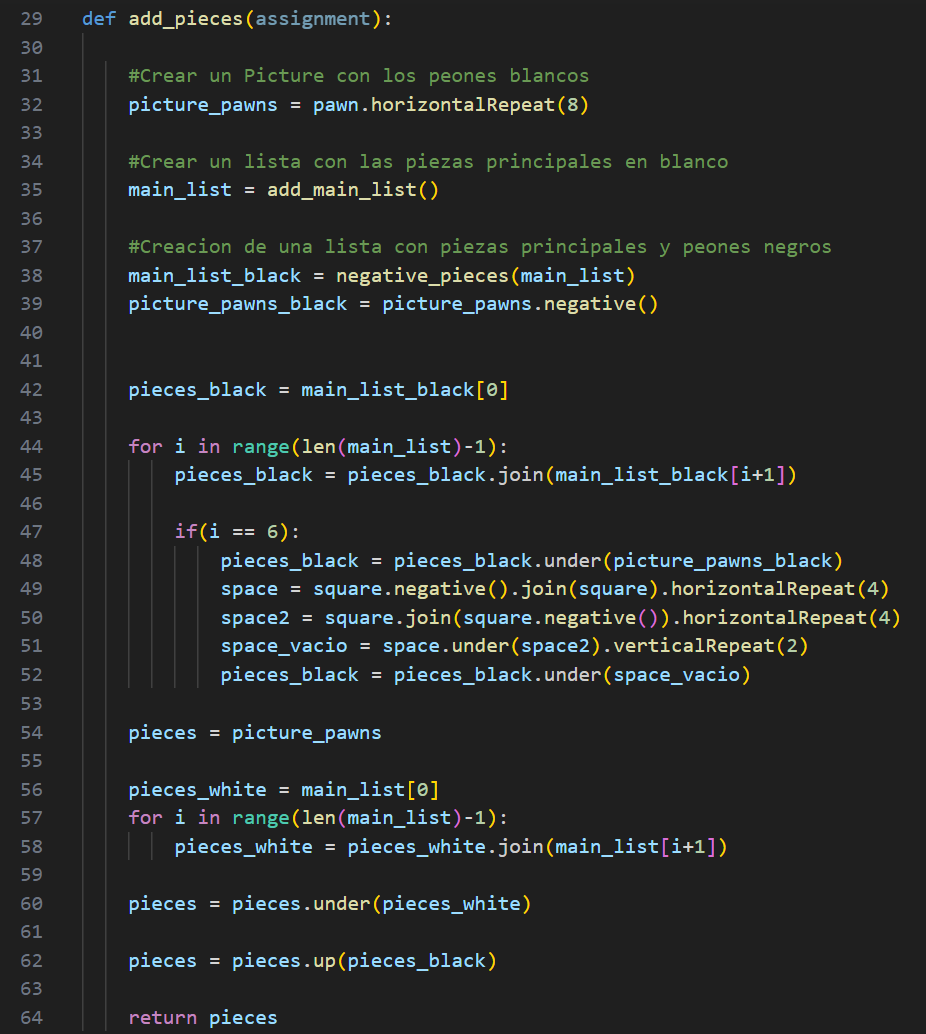
\includegraphics[width=0.55\textwidth,keepaspectratio]{img/cap16_2.png}
		%\includesvg{img/automata.svg}
		%\label{img:mot2}
		%\caption{Product backlog.}
	\end{figure}
	
	Para finalizar se crea el tablero completo con la misma lógica del ejercicio anterior, y posteriormente se hace un llamado a la función “add\_pieces” creándose un Picture pieces, y finalmente se dibujan ambos, en el orden de creación.
	
	\begin{figure}[H]
		\centering
		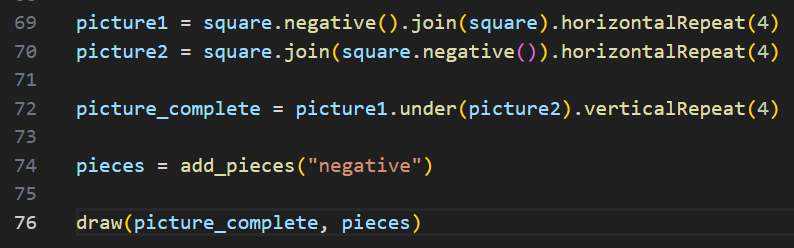
\includegraphics[width=0.55\textwidth,keepaspectratio]{img/cap16_3.png}
		%\includesvg{img/automata.svg}
		%\label{img:mot2}
		%\caption{Product backlog.}
	\end{figure}
	
	\begin{figure}[H]
		\centering
		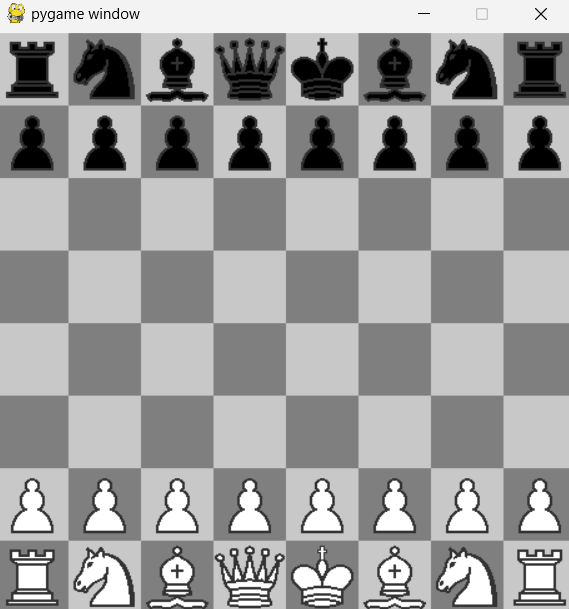
\includegraphics[width=0.55\textwidth,keepaspectratio]{img/Picture G.png}
		%\includesvg{img/automata.svg}
		%\label{img:mot2}
		%\caption{Product backlog.}
	\end{figure}
	
	\subsection{Estructura de laboratorio 04}
	\begin{itemize}	
		\item El contenido que se entrega en este laboratorio es el siguiente:
	\end{itemize}
	
\begin{lstlisting}[style=ascii-tree]
	Pweb2-Lab03/
	|-- Laboratorio 04
	|   |-- chessPictures.py
	|   |-- colors.py
	|   |-- Ejercicio2a.py
	|   |-- Ejercicio2b.py
	|   |-- Ejercicio2c.py
	|   |-- Ejercicio2d.py
	|   |-- Ejercicio2e.py
	|   |-- Ejercicio2f.py
	|   |-- Ejercicio2g.py
	|   |-- interpreter.py
	|   |-- picture.py
	|   |-- pieces.py
	|   |-- prac.py
	|   |
	|   |-- __pycache__
	|       |-- chessPictures.cpython-310.pyc
	|       |-- colors.cpython-310.pyc
	|       |-- interpreter.cpython-310.pyc
	|       |-- picture.cpython-310.pyc
	|       |-- pieces.cpython-310.pyc
	|
	|-- Latex
	|   |-- Laboratorio_04.aux
	|   |-- Laboratorio_04.log
	|   |-- Laboratorio_04.out
	|   |-- Laboratorio_04.pdf
	|   |-- Laboratorio_04.synctex.gz
	|   |-- Laboratorio_04.tex
	|   |
	|   |-- img
	|   |   |-- logo_abet.png
	|   |   |-- logo_episunsa.png
	|   |   |-- logo_unsa.jpg
	|   |   |-- Picture A.png
	|   |   |-- Picture B.png
	|   |   |-- Picture C.png
	|   |   |-- Picture D.png
	|   |   |-- Picture E.png
	|   |   |-- Picture F.png
	|   |   |-- Picture G.png
	|   |   |-- Picture H.png
	|   |
	|   |-- src
	|       |-- horizontalMirror.py
	|       |-- horizontalRepeat.py
	|       |-- join.py
	|       |-- negative.py
	|       |-- rotate.py
	|       |-- under.py
	|       |-- up.py
	|       |-- verticalRepeat.py
\end{lstlisting}       

\subsection{Commits de laboratorio 04}

	\textbf{1er commit:}
	
	\vspace{0.3cm}
	En este commit se copian todos los archivos necesarios para el funcionamiento de la actividad:
	colors.py, interpreter, etc.
	\vspace{0.3cm}

	\begin{figure}[H]
		\centering
		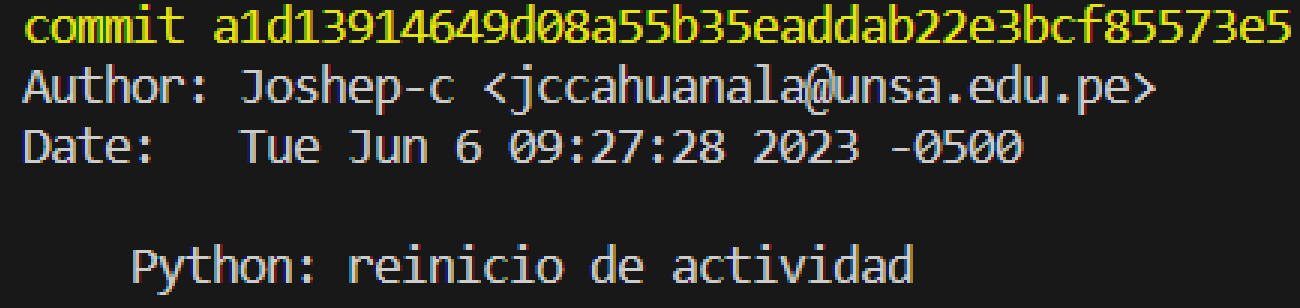
\includegraphics[width=0.55\textwidth,keepaspectratio]{img/commit1.png}
		%\includesvg{img/automata.svg}
		%\label{img:mot2}
		%\caption{Product backlog.}
	\end{figure}
	
	\textbf{2do commit:}
	
	\vspace{0.3cm}
	Implementación del método horizontalMirror en picture.py
	\vspace{0.3cm}
	
	\begin{figure}[H]
		\centering
		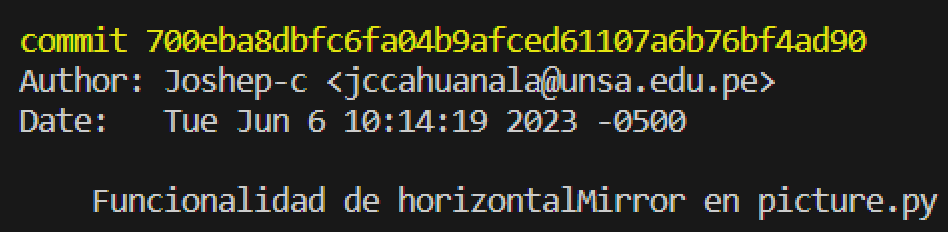
\includegraphics[width=0.55\textwidth,keepaspectratio]{img/commit2.png}
		%\includesvg{img/automata.svg}
		%\label{img:mot2}
		%\caption{Product backlog.}
	\end{figure}
	
	\textbf{3er commit:}
	
	\vspace{0.3cm}
	Implementación de los métodos negative, join, up y under, de manera seguida y directa porque necesitaban mucho razonamiento, principalmente de los dos últimos ya que fue simplemente una agregación de listas.
	\vspace{0.3cm}
	
	\begin{figure}[H]
		\centering
		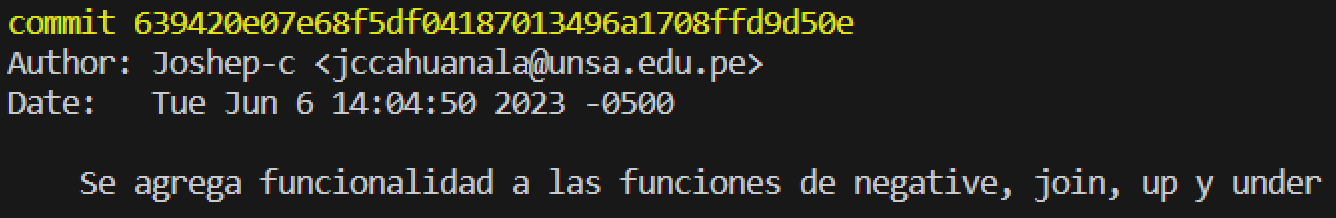
\includegraphics[width=0.55\textwidth,keepaspectratio]{img/commit3.png}
		%\includesvg{img/automata.svg}
		%\label{img:mot2}
		%\caption{Product backlog.}
	\end{figure}
	
	\textbf{4to commit:}
	
	\vspace{0.3cm}
	En este commit se terminó con la implementación de todos los métodos, ósea se completaron los siguientes métodos: horizontalRepeat, verticalRepeat y rotate. De esta manera se completaron los 9 métodos del módulo picture, donde se ubica la clase Picture.
	\vspace{0.3cm}
	
	\begin{figure}[H]
		\centering
		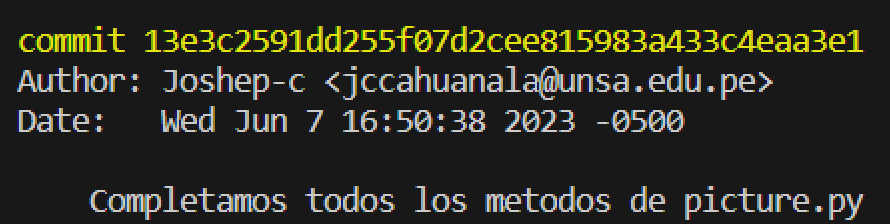
\includegraphics[width=0.55\textwidth,keepaspectratio]{img/commit4.png}
		%\includesvg{img/automata.svg}
		%\label{img:mot2}
		%\caption{Product backlog.}
	\end{figure}
	
	\textbf{5to y 6to commit:}
	
	\vspace{0.3cm}
	Commit de la resolución del ejercicio a, dibujando las 4 piezas de caballo en la ventana del juego. Usando el método draw del módulo interpreter.py.
	\vspace{0.3cm}
	
	\begin{figure}[H]
		\centering
		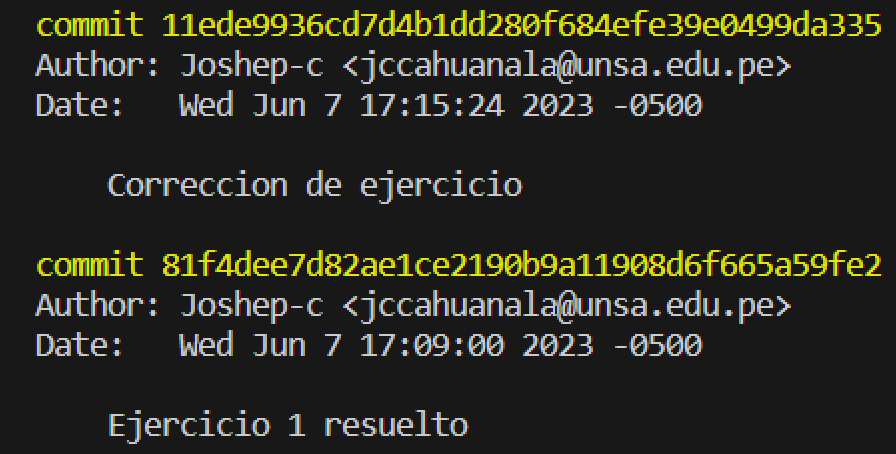
\includegraphics[width=0.55\textwidth,keepaspectratio]{img/commit5-6.png}
		%\includesvg{img/automata.svg}
		%\label{img:mot2}
		%\caption{Product backlog.}
	\end{figure}
	
	\textbf{7mo commit:}
	
	\vspace{0.3cm}
	Commit de la resolución del ejercicio a, dibujando las 4 piezas de caballo en la ventana del juego.
	\vspace{0.3cm}
	
	\begin{figure}[H]
		\centering
		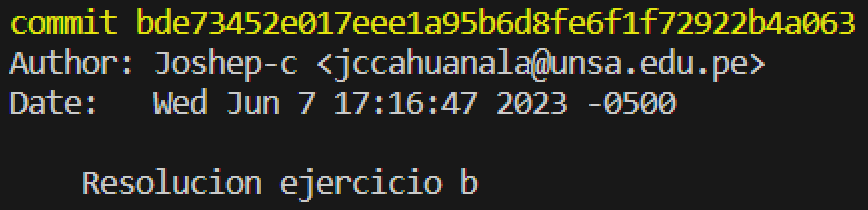
\includegraphics[width=0.55\textwidth,keepaspectratio]{img/commit7.png}
		%\includesvg{img/automata.svg}
		%\label{img:mot2}
		%\caption{Product backlog.}
	\end{figure}
	
	\textbf{8vo commit:}
	
	\vspace{0.3cm}
	Se guardó la resolución del ejercicio 3, del dibujo de las piezas “queen” cuatro veces en horizontal.
	\vspace{0.3cm}
	
	\begin{figure}[H]
		\centering
		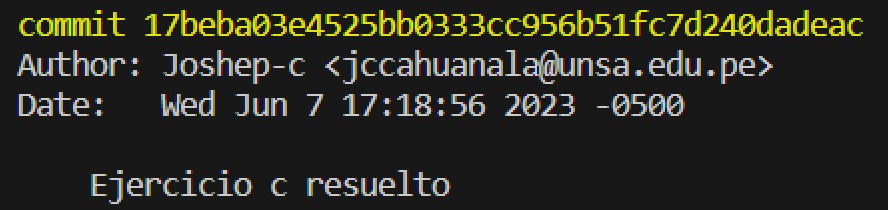
\includegraphics[width=0.55\textwidth,keepaspectratio]{img/commit8.png}
		%\includesvg{img/automata.svg}
		%\label{img:mot2}
		%\caption{Product backlog.}
	\end{figure}
	
	\textbf{9no commit:}
	
	\vspace{0.3cm}
	Culminación del ejercicio d, en la cual se dibuja la primera línea del tablero, intercalando “square” de diferentes colores.
	\vspace{0.3cm}
	
	\begin{figure}[H]
		\centering
		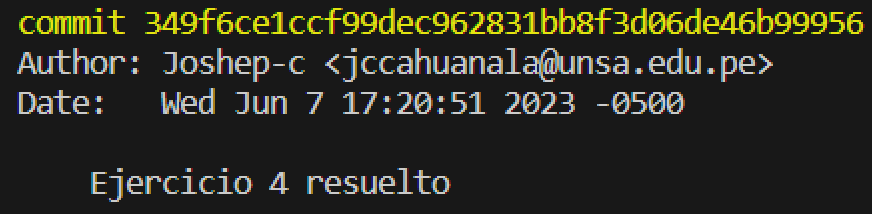
\includegraphics[width=0.55\textwidth,keepaspectratio]{img/commit9.png}
		%\includesvg{img/automata.svg}
		%\label{img:mot2}
		%\caption{Product backlog.}
	\end{figure}
	
	\textbf{10mo commit:}
	
	\vspace{0.3cm}
	Se guarda el código para el ejercicio e, lo mismo que el anterior pero invertido.
	\vspace{0.3cm}
	
	\begin{figure}[H]
		\centering
		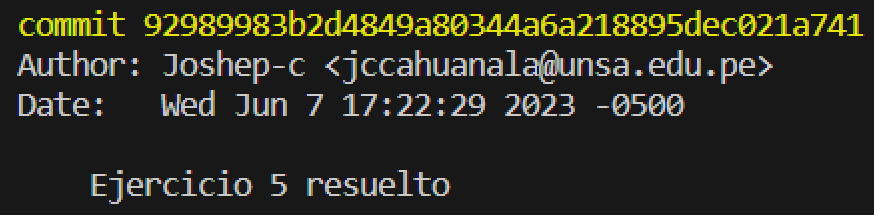
\includegraphics[width=0.55\textwidth,keepaspectratio]{img/commit10.png}
		%\includesvg{img/automata.svg}
		%\label{img:mot2}
		%\caption{Product backlog.}
	\end{figure}
	
	\textbf{11vo commit:}
	
	\vspace{0.3cm}
	Para este commit se guardó el ejercicio F, el cual consiste en mezclar las dos filas creadas en los anteriores ejercicios y duplicarlas hacia abajo de manera intercalada.
	\vspace{0.3cm}
	
	\begin{figure}[H]
		\centering
		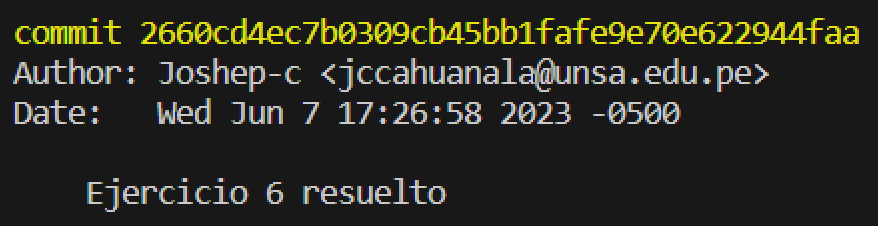
\includegraphics[width=0.55\textwidth,keepaspectratio]{img/commit11.png}
		%\includesvg{img/automata.svg}
		%\label{img:mot2}
		%\caption{Product backlog.}
	\end{figure}
	
	\textbf{12vo commit:}
	
	\vspace{0.3cm}
	Modificación de los módulos colors.py e interpreter.py, el primero para crear una transparencia donde anteriormente se tornaba de azul en “ “ (los espacios), y el segundo para poder ingresar más de un argumento al método draw del módulo interpreter.py.
	\vspace{0.3cm}
	
	\begin{figure}[H]
		\centering
		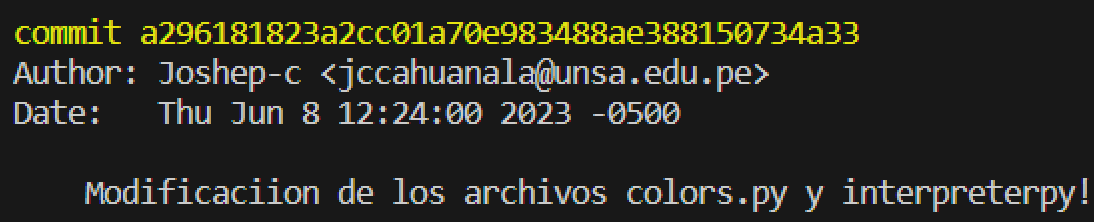
\includegraphics[width=0.55\textwidth,keepaspectratio]{img/commit12.png}
		%\includesvg{img/automata.svg}
		%\label{img:mot2}
		%\caption{Product backlog.}
	\end{figure}
	
	\textbf{13vo commit:}
	
	\vspace{0.3cm}
	Se agregan las funciones negative\_pieces, add\_pieces y add\_pawn. La primera para recibir una lista de Picture y mediante un for, cambiando el color por su perspectivismo negativo de cada elemento, por el método negative; el segundo es una función general para crear las piezas del tablero además de crear los espacios “square” entre las fichas blancas y negras; y el tercero para crear y retornar los peones o pawns. Además de modificar el tipo de retorno del método verticalMirror del módulo picture.py.
	\vspace{0.3cm}
	
	\begin{figure}[H]
		\centering
		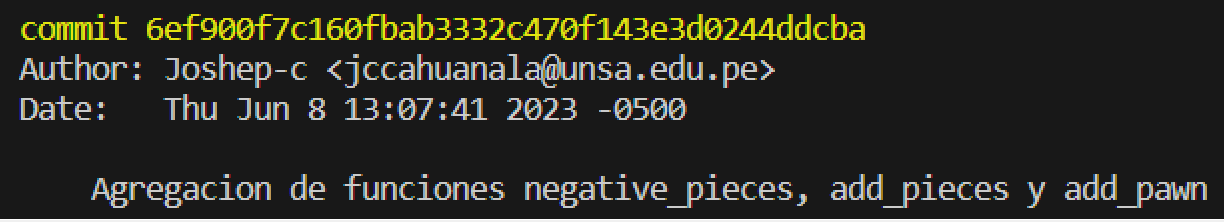
\includegraphics[width=0.55\textwidth,keepaspectratio]{img/commit13.png}
		%\includesvg{img/automata.svg}
		%\label{img:mot2}
		%\caption{Product backlog.}
	\end{figure}
	
	\textbf{14vo commit:}
	
	\vspace{0.3cm}
	En este penúltimo commit se guarda la agregación de la función add\_main\_list, la cual retorna un arreglo con las piezas principales del ajedrez, excepto los peones, y de color blanco, osea por defecto.
	\vspace{0.3cm}
	
	\begin{figure}[H]
		\centering
		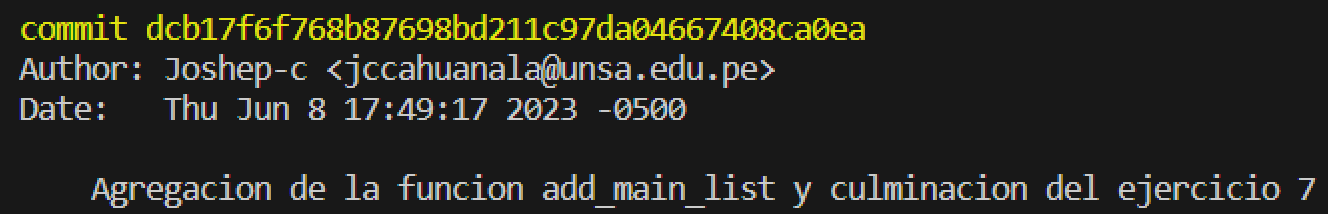
\includegraphics[width=0.55\textwidth,keepaspectratio]{img/commit14.png}
		%\includesvg{img/automata.svg}
		%\label{img:mot2}
		%\caption{Product backlog.}
	\end{figure}
	
	\textbf{15vo commit:}
	
	\vspace{0.3cm}
	En este último commit se modificó el tamaño de la ventana para que se ajuste a las dimensiones del tablero en sí, ya que aparecía espacio sobrante de color azul, osea con espacios. Además se estaban modificando algunos detalles y nombres de variables en los diferentes módulos y funciones.
	\vspace{0.3cm}
	
	\begin{figure}[H]
		\centering
		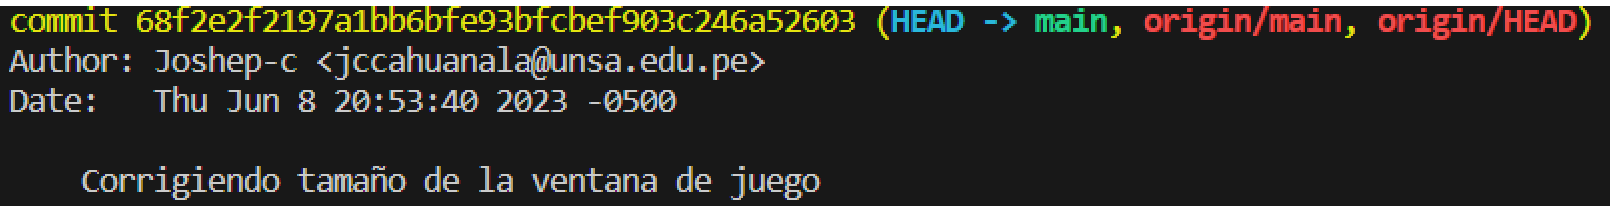
\includegraphics[width=0.55\textwidth,keepaspectratio]{img/commit15.png}
		%\includesvg{img/automata.svg}
		%\label{img:mot2}
		%\caption{Product backlog.}
	\end{figure}


	\section{Cuestionario:}
	
	\textbf{¿Qué son los archivos *.pyc?}
	
	\vspace{0.3cm}
	Los archivos ".pyc" son archivos de código compilado en Python que se generan automáticamente al ejecutar o importar un archivo ".py". Contienen el código fuente compilado a un formato más eficiente para mejorar el rendimiento en ejecuciones futuras del programa. Estos archivos son específicos de la versión y configuración del intérprete de Python utilizado y pueden volverse obsoletos si cambias la versión o ciertas configuraciones.
	\vspace{0.3cm}
	
	\textbf{¿Para qué sirve el directorio pycache?}
	
	\vspace{0.3cm}
	El directorio "pycache" es una carpeta especial que se crea automáticamente cuando ejecutas o importas archivos de Python. En esta carpeta se guardan los archivos que contienen el código compilado del programa para que se ejecuten más rápidamente en el futuro. El directorio "pycache" ayuda a organizar y separar estos archivos compilados de los archivos fuente, facilitando el mantenimiento del proyecto y mejorando el rendimiento de tu programa.
	\vspace{0.3cm}
	
	\textbf{¿Cuáles son los usos y lo que representa el subguión en Python?}
	
	\vspace{0.3cm}
	El subguión (\_) en Python tiene varios usos y significados adicionales además de ser utilizado en constructores y para indicar métodos privados de una clase (como en la clase Picture). Algunos de estos usos incluyen:
	
	\begin{itemize}
		\item \textbf{Traducción de cadenas:} En la función str.maketrans() o en el método str.translate(), puedes utilizar el subguión para indicar que un carácter debe ser eliminado o dejado sin cambios durante una operación de traducción de cadenas.
	\end{itemize}
	
	\begin{lstlisting}[language=bash,caption={Ejemplo}][H]
		translation_table = str.maketrans("aeiou","_____")
		resultado = "Hola, mundo!".translate(translation_table)
		print(resultado)			
		
		Ouput >>  H_l_, m_nd_!
	\end{lstlisting}		
	
	\begin{itemize}
		\item \textbf{Ignorar valores en desempaquetado:} Al desempaquetar una secuencia o iterador, puedes utilizar el subguión para ignorar los valores que no necesitas. 
	\end{itemize}
	
	\begin{lstlisting}[language=bash,caption={Ejemplo}][H]
		a, _, c = (1, 2, 3)
	\end{lstlisting}	
	
	\vspace{0.3cm}
	
	\clearpage
	
	\section{\textcolor{red}{Rúbricas}}
	
	\subsection{\textcolor{red}{Entregable Informe}}
	\begin{table}[H]
		\caption{Tipo de Informe}
		\setlength{\tabcolsep}{0.5em} % for the horizontal padding
		{\renewcommand{\arraystretch}{1.5}% for the vertical padding
			\begin{tabular}{|p{3cm}|p{12cm}|}
				\hline
				\multicolumn{2}{|c|}{\textbf{\textcolor{red}{Informe}}}  \\
				\hline 
				\textbf{\textcolor{red}{Latex}} & \textcolor{blue}{El informe está en formato PDF desde Latex,  con un formato limpio (buena presentación) y facil de leer.}   \\ 
				\hline 
				
				
			\end{tabular}
		}
	\end{table}
	
	\subsection{\textcolor{red}{Rúbrica para el contenido del Informe y demostración}}
	\begin{itemize}			
		\item El alumno debe marcar o dejar en blanco en celdas de la columna \textbf{Checklist} si cumplio con el ítem correspondiente.
		\item Si un alumno supera la fecha de entrega,  su calificación será sobre la nota mínima aprobada, siempre y cuando cumpla con todos lo items.
		\item El alumno debe autocalificarse en la columna \textbf{Estudiante} de acuerdo a la siguiente tabla:
		
		\begin{table}[ht]
			\caption{Niveles de desempeño}
			\begin{center}
				\begin{tabular}{ccccc}
					\hline
					& \multicolumn{4}{c}{Nivel}\\
					\cline{1-5}
					\textbf{Puntos} & Insatisfactorio 25\%& En Proceso 50\% & Satisfactorio 75\% & Sobresaliente 100\%\\
					\textbf{2.0}&0.5&1.0&1.5&2.0\\
					\textbf{4.0}&1.0&2.0&3.0&4.0\\
					\hline
				\end{tabular}
			\end{center}
		\end{table}	
		
	\end{itemize}
	
	\begin{table}[H]
		\caption{Rúbrica para contenido del Informe y demostración}
		\setlength{\tabcolsep}{0.5em} % for the horizontal padding
		{\renewcommand{\arraystretch}{1.5}% for the vertical padding
			%\begin{center}
			\begin{tabular}{|p{2.7cm}|p{7cm}|x{1.3cm}|p{1.2cm}|p{1.5cm}|p{1.1cm}|}
				\hline
				\multicolumn{2}{|c|}{Contenido y demostración} & Puntos & Checklist & Estudiante & Profesor\\
				\hline
				\textbf{1. GitHub} & Hay enlace URL activo del directorio para el  laboratorio hacia su repositorio GitHub con código fuente terminado y fácil de revisar. &2 &X &2 & \\ 
				\hline
				\textbf{2. Commits} &  Hay capturas de pantalla de los commits más importantes con sus explicaciones detalladas. (El profesor puede preguntar para refrendar calificación). &4 &X &4 & \\ 
				\hline 
				\textbf{3. Código fuente} &  Hay porciones de código fuente importantes con numeración y explicaciones detalladas de sus funciones. &2 &X &2 & \\ 
				\hline 
				\textbf{4. Ejecución} & Se incluyen ejecuciones/pruebas del código fuente  explicadas gradualmente. &2 &X &2 & \\ 
				\hline			
				\textbf{5. Pregunta} & Se responde con completitud a la pregunta formulada en la tarea.  (El profesor puede preguntar para refrendar calificación).  &2 &X &2 & \\ 
				\hline	
				\textbf{6. Fechas} & Las fechas de modificación del código fuente estan dentro de los plazos de fecha de entrega establecidos. &2 &X &2 & \\ 
				\hline 
				\textbf{7. Ortografía} & El documento no muestra errores ortográficos. &2 &X &2 & \\ 
				\hline 
				\textbf{8. Madurez} & El Informe muestra de manera general una evolución de la madurez del código fuente,  explicaciones puntuales pero precisas y un acabado impecable.   (El profesor puede preguntar para refrendar calificación).  &4 &X &4 & \\ 
				\hline
				\multicolumn{2}{|c|}{\textbf{Total}} &20 & &20 & \\ 
				\hline
			\end{tabular}
			%\end{center}
			%\label{tab:multicol}
		}
	\end{table}
	
	\clearpage
	
	
\clearpage

\section{Referencias}
\begin{itemize}			
	\item \url{https://www.w3schools.com/java/default.asp}
	\item \url{https://www.geeksforgeeks.org/insertion-sort/}
	\item \url{https://github.com/Joshep-c/PW2LAB.git}
\end{itemize}	
	
%\clearpage
%\bibliographystyle{apalike}
%\bibliographystyle{IEEEtranN}
%\bibliography{bibliography}
			
\end{document}